\documentclass[a4paper]{article}
\usepackage[spanish]{babel}
\usepackage[utf8]{inputenc}
\usepackage[T1]{fontenc}
\usepackage{charter}  % tipografia
\usepackage{graphicx}
\usepackage{float}
\usepackage{amsmath, amsthm, amssymb}
\usepackage{inconsolata}
\usepackage{clrscode}
\usepackage{underscore}
\usepackage{caratula}
\usepackage{listings}
\usepackage{array}

\usepackage[a4paper, margin=2.54cm]{geometry}

\usepackage{fancyhdr}
\pagestyle{fancy}

%\renewcommand{\chaptermark}[1]{\markboth{#1}{}}
%\renewcommand{\sectionmark}[1]{\markright{\thesection\ - #1}}

%\fancyhf{}

%\fancyhead[LO]{Sección \rightmark} % \thesection\ 
\fancyfoot{}
\lfoot{\small{Integrantes}}
\rfoot{\thepage}

%\renewcommand{\headrulewidth}{0.5pt}
%\renewcommand{\footrulewidth}{0.5pt}
%\setlength{\hoffset}{-0.8in}
%\setlength{\textwidth}{16cm}
%\setlength{\hoffset}{-1.1cm}
%\setlength{\textwidth}{16cm}
%\setlength{\headsep}{0.5cm}
%\setlength{\textheight}{25cm}
%\setlength{\voffset}{-0.7in}
%\setlength{\headwidth}{\textwidth}
%\setlength{\headheight}{13.1pt}

%\renewcommand{\baselinestretch}{1.1}  % line spacing
\linespread{1.2}



\lstset{language=[x64]Assembler}
\lstset{basicstyle=\ttfamily\small}
\lstset{frame=single,tabsize=4}
\lstset{captionpos=b}
\lstset{inputencoding=utf8}
\lstset{numbers=left}
\lstset{texcl=true}
\lstset{escapeinside={(*@}{@*)}}
\renewcommand{\lstlistingname}{Código}


\begin{document}

\materia{Algoritmos y Estructuras de Datos III}
\titulo{TP1}

\integrante{Alonso Tomás}{396/16}{tomasalonso96@gmail.com}

\maketitle
\newpage

\tableofcontents
\newpage

\section{Introducción}

El trabajo realizado implementa la simulacion de flujo de fluidos basada en las
ecuaciones de Navier-Stokes, la eleccion de utilizar estas ecuaciones es porque
se consigue un resultado que no es numericamente preciso pero es lo
suficientemente estable, simple y fiel a la realidad como para dejar ver lo que
este trabajo intenta observar.



El objetivo final es poder observar las
diferencias de rendimiento de programas en codigo en C comparados con la misma
logica pero implementada en Assembler utilizando el set de instrucciones SSE
propio de los procesadores intel.



En principio se explican las decisiones de implementacion del codigo, ya sean de
comodidad y simpleza o por mejoria de rendimiento, asi como tambien se habla
sobre intentos fallidos por intentar mejorar la performance al utilizar
extensivamente la metodologia SIMD, pero encontrandonos con inconvenientes
inesperados. Tambien se puede observar que es lo que efectivamente realiza el
codigo y como esto influyó en las decisiones tomadas.



Una vez en claro como funciona el programa y porque se decidio hacerlo asi, se
muestra la experimentacion exhaustiva que se hizo para medir las diferencias de
tiempos entre todo el trabajo con las funciones en C en comparacion con todas
las funciones nuevas en assembler, esto en relacion con el rendimiento comparado
entre cada funcion en C con su contraparte en assembler. Con todo esto se puede
ver claramente que implementacion es mas rapida asi como distinguir que
funciones son las que hacen la mayor diferencia en general.

\newpage
\section{Desarrollo}

\subsection{solver_lin_solve}

Como primer enfoque para la implementación de {\it solver_lin_solve\/} se pensó en
leer de a columnas y maximizar la cantidad de posiciones que calculábamos a
la vez, tal como puede apreciarse en la \hbox{\it figura 1\/}.

La principal ventaja de leer de a columnas, es reusar la fila calculada con
anterioridad, evitándose así una relectura a memoria.

Luego, para maximizar la cantidad de posiciones, se usaban los 16 registros {\it
  xmm\/}.
Dando por resultado la lectura de segmentos de matriz de $3\times24$
posiciones simultáneas y el calculo de 22 posiciones nuevas por iteración del
ciclo. En cada iteración se leían 24 posiciones nuevas de la siguiente fila
(siempre manteniéndose en la misma columna de 24 elementos).
Una vez que ya no era posible de a 24, se terminaba de iterar la matriz
calculando de a 2 posiciones.

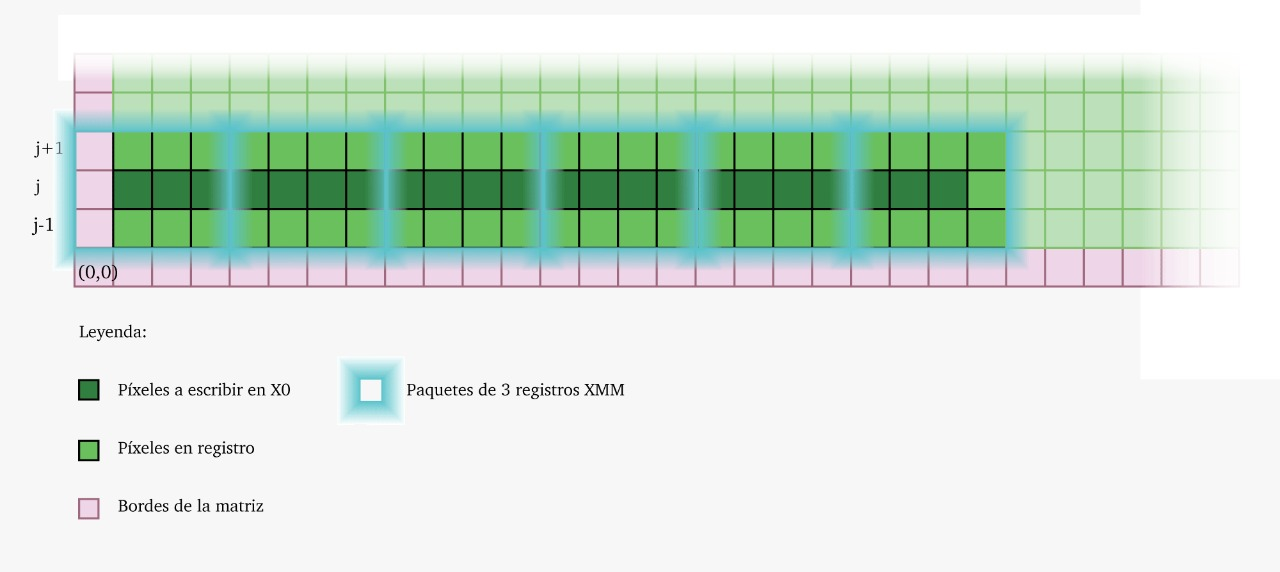
\includegraphics[width=\textwidth]{imagenes/24.jpeg}

Dicha implementación no fue completamente terminada, pero primeras
pruebas de la misma mostraron un rendimiento muy por debajo de lo esperado,
dando solo una leve mejora a la versión C provista por la cátedra (ver más en
resultados (sección piripitruli)).

Por este motivo fue descartada (código en {\it solver_lin_solve_largo.asm\/}
\footnote{El código no presenta errores de {\bf segmentation fault} y puede ser
  ejecutado. Sin embargo, al ser un código {\bf no} finalizado, produce errores
  en el cálculo de fluidos.}).

Entre las hipótesis acerca de la merma de rendimiento pensamos en la extensa
longitud del código de los ciclos y la forma de lectura por columnas de la
matriz que no aprovecha el modo de almacenamiento por filas \footnote{\#define
  IX(i,j) (i+(solver->N+2)*j)}.

\noindent\hfill\rule{0.7\textwidth}{0.4pt}\hfill
\hskip0.3em

Como opción final, se optó leer por medio de iteradores (puntero a la matriz)
que recorran la matriz por filas y calculen de a 2 posiciones a la vez,
$(i,j)$ e $(i+1,j)$.

Usándose la estrategia detallada a continuación para realizar el siguiente
calculo en paralelo, para cada posición de la matriz:

$$x(i,j) = \frac{x_0(i,j) +
  a*\bigl(x(i-1,j)+x(i+1,j)+x(i,j-1)+x(i,j+1)\bigr)}{c}$$

Primero notamos que si separamos en casos $a = 0$ y $a \neq 0$, nos permite que
en el caso $a = 0$, el cálculo se reduzca a:

$$x(i,j) = \frac{x_0(i,j)}{c}$$

Que podemos realizarlo de a 4 posiciones en paralelo por iteración de ciclo,
por medio de un iterador de $x_0$ y un iterador de $x$, en contraposición a
calcular de a 2 posiciones como realizamos en el caso general ($a \neq 0$), que
detallaremos más adelante. Otra ventaja es que el cálculo se reduce a una sola
instrucción (dividir por {\it c\/}).



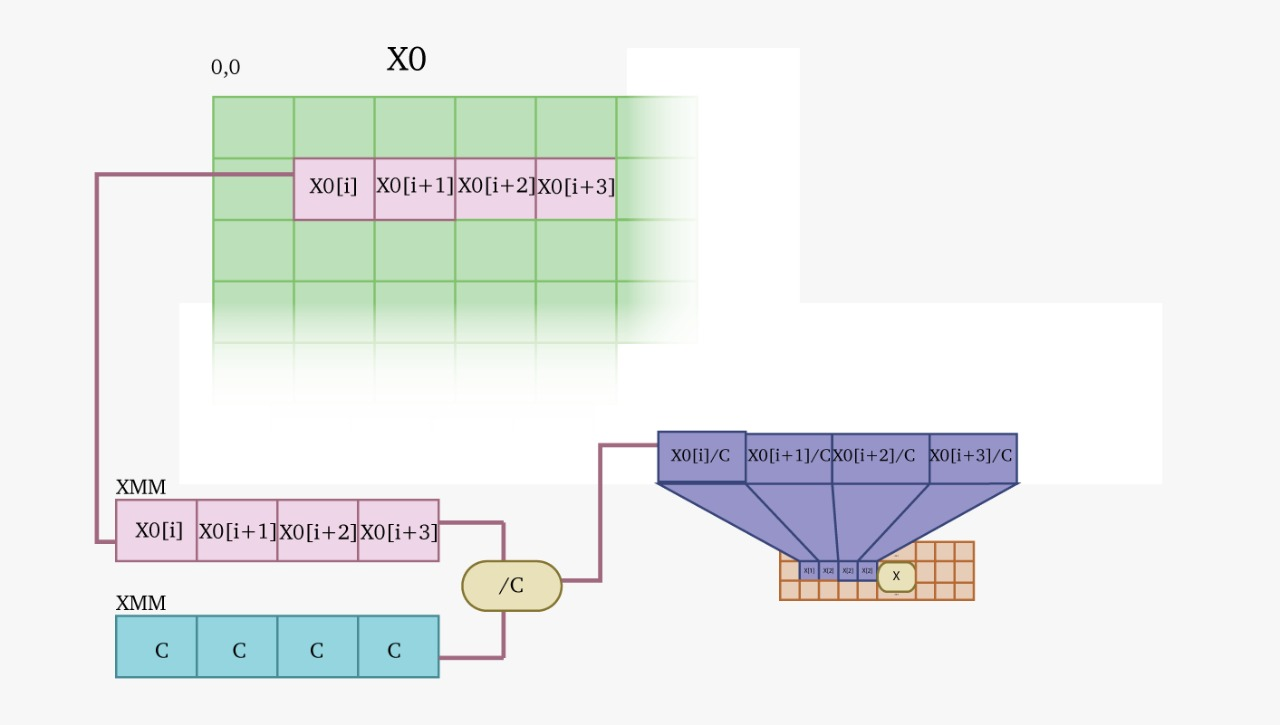
\includegraphics[width=\textwidth]{imagenes/lina0.jpeg}


x0 --> (carga en xmm) | x0[i][j] | x0[i+1][j] | x0[i+2][j] | x0[i+3][j] |
--> (div por c) | x0[i][j]/c | x0[i+1][j]/c | x0[i+2][j]/c | x0[i+3][j]/c |
--> (carga en memoria) x

En el caso $a \neq 0$, se utilizan 4 iteradores que apuntan respectivamente

% iter1_x: x(i,j-1)
% iter2_x: x(i-1,j)
% iter3_x: x(i,j+1)
% iter_x0: x0(i,j)



En cada iteración, se calculan las posiciones $x(i,j)$ y $x(i+1,j)$.
Se leen 2 posiciones a partir de {\it iter1_x\/}, 2 de {\it iter3_x\/}, 2 de
{\it iter_x0\/} y 4 de {\it iter2_x\/}, dando por resultado la carga en
registros {\it xmm\/} de las siguiente posiciones.

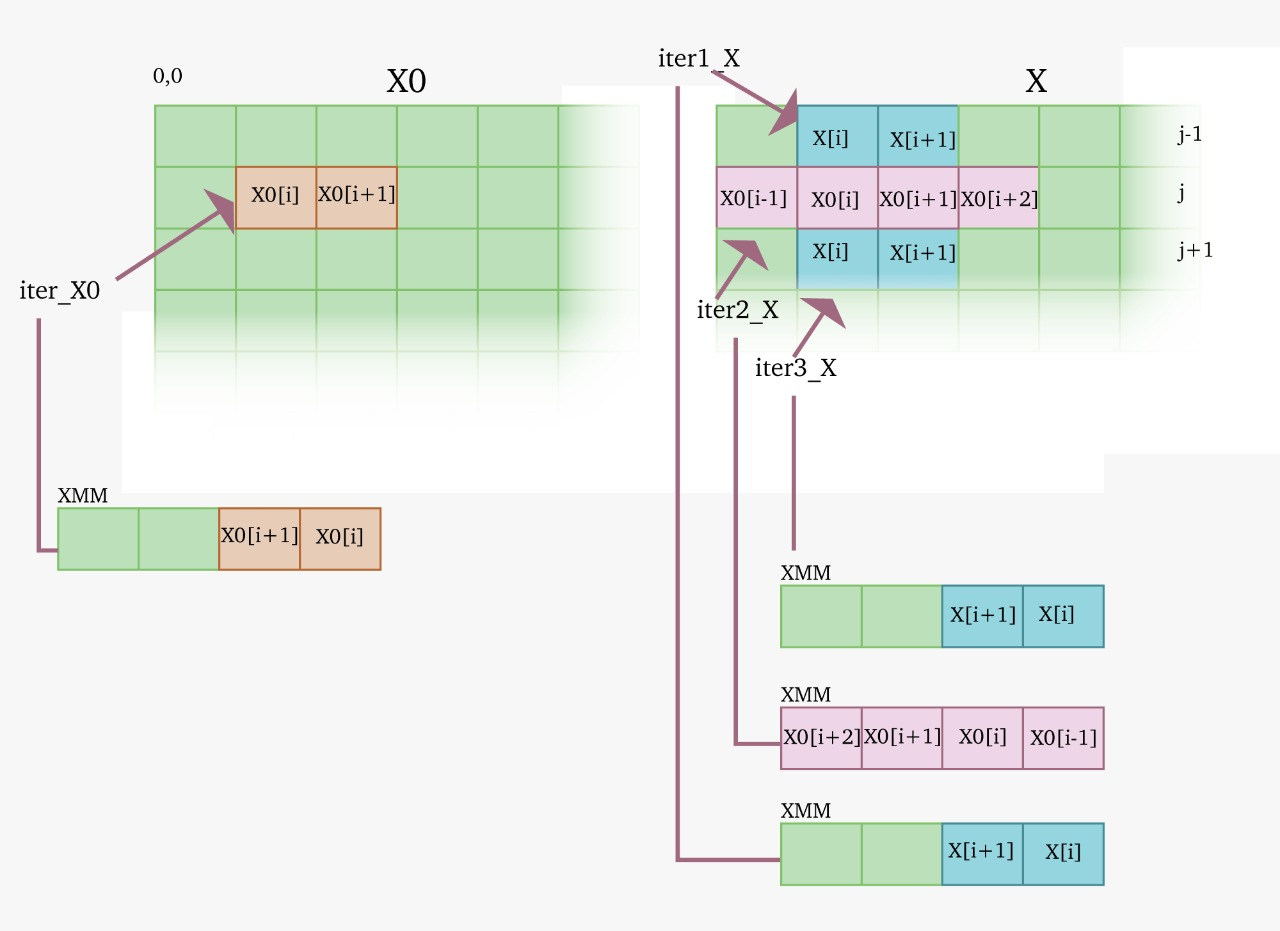
\includegraphics[width=\textwidth]{imagenes/liniter.jpeg}


Consecuentemente, se calculan en paralelo, es decir de a 2 posiciones
simultáneas, la suma

{
\setlength{\abovedisplayskip}{-5pt}
\setlength{\belowdisplayskip}{-5pt}
\begin{align*}
x(i,j) &:= \frac{x_0(i,j)}{a} + x(i+1,j) + x(i,j-1) + x(i,j+1)\\
x(i+1,j) &:= \frac{x_0(i,j)}{a} + x(i+1,j) + x(i,j-1) + x(i,j+1)
\end{align*}
}


para $x(i,j)$ y $x(i+1,j)$ como muestra la figura.

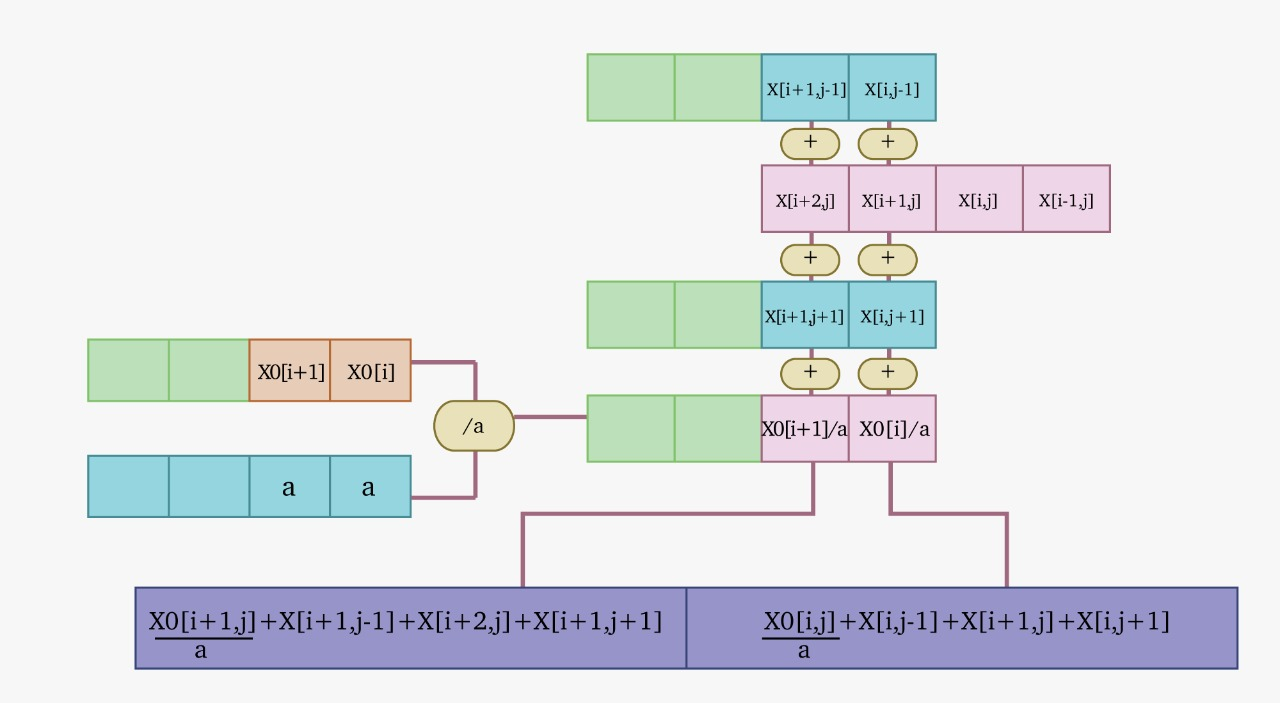
\includegraphics[width=\textwidth]{imagenes/lina11.jpeg}


Luego, se calcula secuencialmente
$$x(i,j) + x(i-1,j)$$
$$x(i,j) / c$$
$$x(i+1,j) + (i,j)$$
$$x(i+1,j) / c$$


FIGURA (diagrama que va mostrando los pasos del algoritmo)

Esto es necesario, debido a que cada posición necesita que la casilla a su
izquierda $x(i-1,j)$ haya sido procesada con anterioridad al sumarse a $x(i,j)$.

Vale la pena aclarar que la casilla $x(i,j-1)$ también debe haber sido procesada al
momento de su suma, pero debido a la manera en que se recorre la matriz, al
leerse la posición $x(i,j-1)$, ya fue calculada con anterioridad.

Por último, se incrementan en dos posiciones los iteradores y se sigue con una
nueva iteración del ciclo hasta completar la matriz.


Esta solución, en principio menos óptima ya que debía leerse 3 veces cada
posición de memoria (ver figura tanto), aprovecha mucho mejor el principio de
localidad en caché, tanto para el código (al ser mucho más compacto), como para
los datos (al recorrer la matriz por filas).

Quedó en el tintero aclarar el por qué las posiciones de memoria se leen 3
veces. Esto ocurre porque si en una iteración se leen las posiciones de $x$
$\bigl[(i,j)|(i+1,j)|(i+2,j)|(i+3,j)\bigr]$, en la siguiente se leen
$\bigl[(i+2,j)|(i+3,j)|(i+4,j)|(i+5,j)\bigr]$, releyéndose las posiciones
$\bigl[(i+2,j)|(i+3,j)\bigr]$. Luego las posiciones
$\bigl[(i+2,j-1)|(i+3,j-1)\bigr]$ también fueron calculadas anteriormente,
leyéndose por tercera vez.

FIGURA |x(i,j)|x(i+1,j)  |x(i+2,j)  |x(i+3,j)  |x(i+4,j)|x(i+5,j)|
                         |x(i+2,j-1)|x(i+3,j-1)|
(poner i+2 e i+3 de otro color que resalte)

Esta desventaja fue superada guardando $x(i+2,j)$ y $x(i+3,j)$ de la iteración
anterior en la parte baja del registro y cargando $x(i+4,j)$ e $x(i+5,j)$ en la parte
alta del registro con {\it movhps\/}\footnote{movhps: carga las posiciones 2 y 3
del registro $xmm = [3|2|1|0]$} sin ninguna modificación extra al algoritmo utilizado.

% Se descartó también la posibilidad de maximizar la cantidad de posiciones
% cargadas al mismo tiempo en los registros,


\subsection{solver_set_bnd}

Para la función {\it solver_set_bnd\/} se desglosó el ciclo en casos $b = 1$,
$b = 2$ y $b \neq 1 \land b \neq 2$.

Al hacerlo, se evita realizar comparaciones dentro del ciclo. Quedando por
resultado un ciclo que por cada iteración calcula lo siguiente:

\begin{center}
  \begin{tabular}{| >{\centering\arraybackslash}m{2in} | >{\centering\arraybackslash}m{2in} | >{\centering\arraybackslash}m{2in} |}
    \hline
    $b = 1$              & $b = 2$              & $b \neq 1 \land b \neq 2$ \\\hline
{
\setlength{\abovedisplayskip}{0pt}
\setlength{\belowdisplayskip}{0pt}
\begin{align*}
  x(0,i) &:= -x(1,i)\\ x(n+1,i) &:= -x(n,i)\\  x(i,0) &:= x(i,1)\\ x(i,n+1) &:= x(i,n)
\end{align*}
} & {
\setlength{\abovedisplayskip}{0pt}
\setlength{\belowdisplayskip}{0pt}
\begin{align*}
  x(0,i) &:= x(1,i)\\ x(n+1,i) &:= x(n,i)\\ x(i,0) &:= -x(i,1)\\ x(i,n+1) &:= -x(i,n)
\end{align*}
} & {
\setlength{\abovedisplayskip}{0pt}
\setlength{\belowdisplayskip}{0pt}
\begin{align*}
  x(0,i) &:= x(1,i)\\ x(n+1,i) &:= x(n,i)\\  x(i,0) &:= x(i,1)\\ x(i,n+1) &:= x(i,n)
\end{align*}} \\\hline
  \end{tabular}
\end{center}

Se usan 4 iteradores y 1 ciclo que itera n veces, calculándose por cada
iteración una nueva posición.
Estos iteradores son {\it upper\/}, {\it bottom\/}, {\it left\/} y {\it right_n\/}.
Y recorren respectivamente,

FIGURA (cuadrito con bordes y nombres del iterador en cada uno)

Por último se realizan los últimos calculos de la misma forma que el código
original

{
\setlength{\abovedisplayskip}{-5pt}
\setlength{\belowdisplayskip}{-20pt}
\begin{align*}
  x(0  ,0  ) &:= 0.5\cdot\bigl(x(1,0  )+x(0  ,1)\bigr)\\
  x(0  ,n+1) &:= 0.5\cdot\bigl(x(1,n+1)+x(0  ,n)\bigr)\\
  x(n+1,0  ) &:= 0.5\cdot\bigl(x(n,0  )+x(n+1,1)\bigr)\\
  x(n+1,n+1) &:= 0.5\cdot\bigl(x(n,n+1)+x(n+1,n)\bigr)\\
\end{align*}
}

Notar que se usa un iterador {\it upper_n\/} ubicado en la fila $n$ en vez
de la $n+1$, esto es debido al formato en que pueden indexarse las direcciones
en {\it intel\/} donde solo se pueden sumar registros y no restarse. En el caso
de haberse optado por un iterador de la fila $n+1$, la siguientes líneas
\footnote{Línea 120 y 121, {\it solver_set_bnd.asm\/}}

\lstset{numbers=none}
\begin{lstlisting}
  mov aux_edx, [upper_n]            ; aux := x[i][N]
  mov [upper_n + lon_fila], aux_edx ; x[i][N+1] := x[i][N]
\end{lstlisting}
deberían ser idealmente
\begin{lstlisting}
  mov aux_edx, [upper - lon_fila]   ; aux := x[i][N]
  mov [upper], aux_edx              ; x[i][N+1] := x[i][N]
\end{lstlisting}

Como la operación no está permitida, la resta debería realizarse anteriormente
en un registro auxiliar. Para evitar esto y aprovechar el modo de
direccionamiento de {\it intel\/}, usamos un iterador a la posición $n$.


\subsection{solver_project}

En esta función se utilizó la misma forma de recorrer la matriz por filas
adoptada en {\it solver_lin_solve\/} (ver blabla), los motivos son los mismos,
aprovechar el principio de localidad en caché.

El calculo a realizar es

{
\setlength{\abovedisplayskip}{-5pt}
\setlength{\belowdisplayskip}{-10pt}
\begin{align*}
  div(i,j) &:= \frac{-0.5 \cdot \bigl(u(i+1,j)-u(i-1,j)+v(i,j+1)-v(i,j-1)\bigr)}{n}\\
  p(i,j)   &:= 0
\end{align*}
}

En primer lugar, para el primer ciclo se utilizan los iteradores {\it div\/},
{\it u\/}, {\it v1\/} y {\it v2\/}.
% FIGURA iteradores
% div: div(i,j)
% u: u(i-1,j)
% v1: v(i,j-1)
% v2: v(i,j+1)
Y se calcula de a 2 posiciones por iteración. Leyendo 4 posiciones de {\it u\/},
2 de {\it v1\/} y 2 de {\it v2\/}. Realizando el cálculo como indica la figura,

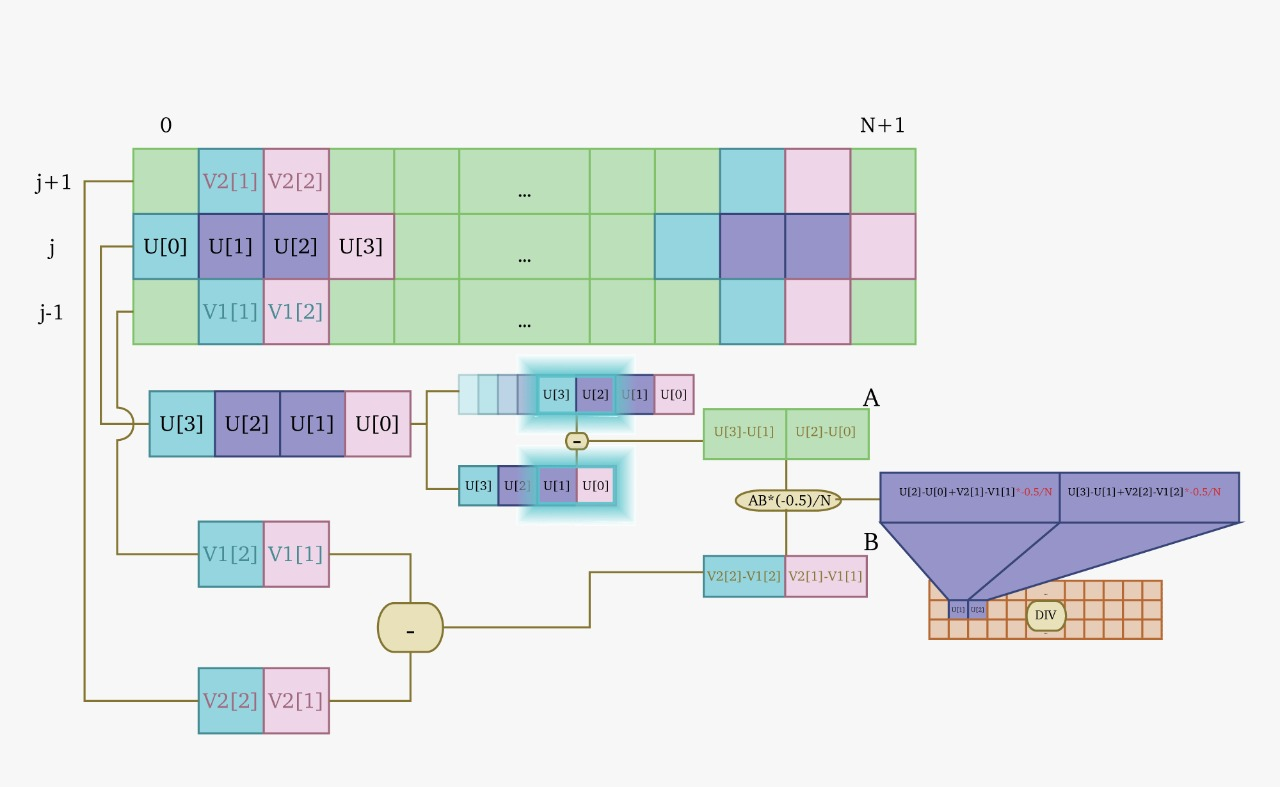
\includegraphics[width=\textwidth]{imagenes/div.jpeg}

Por último, se incrementan los iteradores en 2 posiciones y se da paso a la
siguiente iteración.

Para el segundo ciclo, donde debe calcularse

{
\setlength{\abovedisplayskip}{-5pt}
\setlength{\belowdisplayskip}{-10pt}
\begin{align*}
  u(i,j) &:= u(i,j) - 0.5n\cdot\bigl(p(i+1,j)-p(i-1,j)\bigr)\\
  v(i,j) &:= v(i,j) - 0.5n\cdot\bigl(p(i,j+1)-p(i,j-1)\bigr)
\end{align*}
}

se optó por separar el ciclo en dos diferentes, en el primero se calcula
{\it u\/} y en el segundo se calcula {\it v\/}.

Esto conlleva la ventaja de poder calcular de a 4 posiciones en paralelo para
{\it v\/} y sortear la limitación de calcular de a 2 posiciones debido al
calculo de {\it u\/} como se explicará a continuación.

La estrategia utilizada para el ciclo de {\it u\/} es usar 2 iteradores, {\it
  iter_p\/} e {\it iter_u\/}.

% iter_p: p[i-1][j]
% iter_u: u[i][j]

\begin{center}
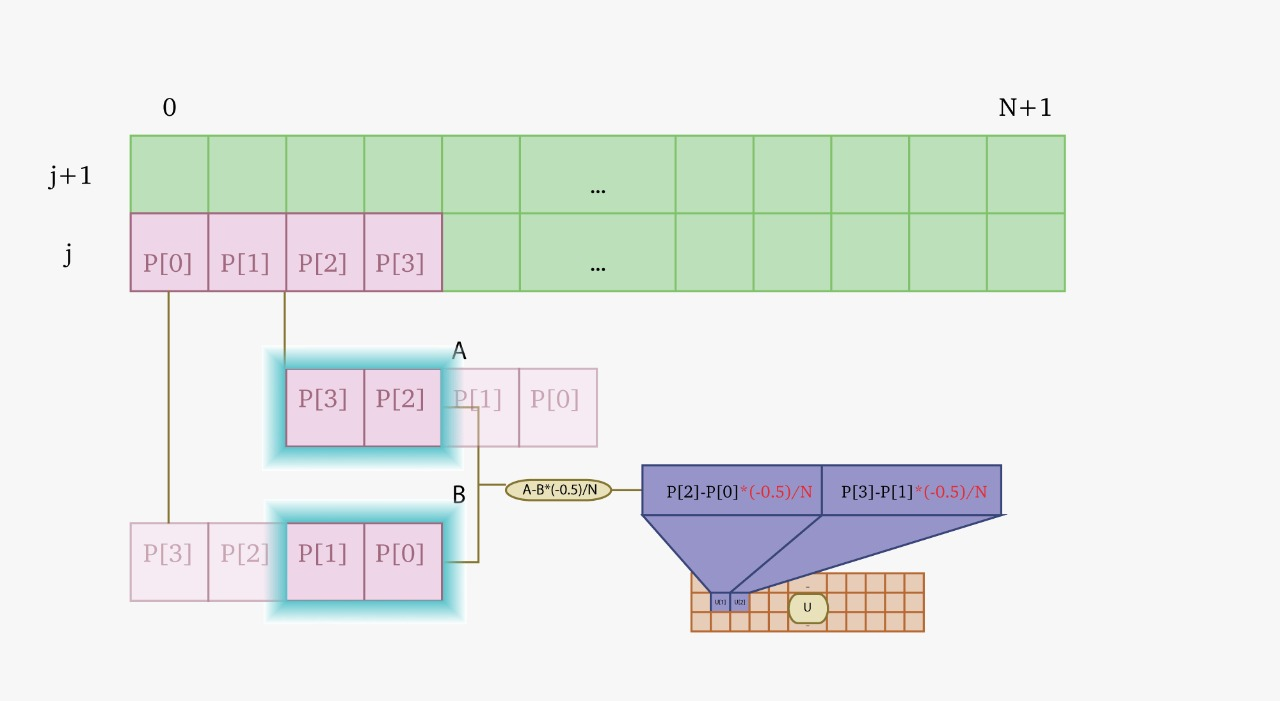
\includegraphics[width=0.7\textwidth]{imagenes/u.jpeg}
\end{center}

En cada iteración se leen 4 posiciones de {\it p\/} y se procesan 2 posiciones
de {\it u\/}.

Diagrama (muestra como calcula paralelamente u)

La estrategia utilizada para el ciclo de {\it v\/} es usar 3 iteradores, {\it
  iter1_p\/}, {\it iter2_p\/} e {\it iter_v}.

% iter1_p: p[i][j-1]
% iter2_p: p[i][j+1]
% iter_v: v[i][j]

Figura (muestra donde se ubican los iteradores)

En cada iteración se leen 4 posiciones de {\it p\/}, 4 de {\it p\/} y se
procesan 4 posiciones de {\it u\/}.

Diagrama (muestra como calcula paralelamente v)

\newpage
\section{Resultados}

En esta seccion se va a hablar de todos los experimentos realizados para poder observar los distintos
comportamientos del programa, ya sea en cuanto a tiempos como en diferencias de resultado, con
las distintas funciones implementadas.

En primer lugar se trabaja el desempeño en tiempo del programa con distintas configuraciones
que seran explicadas en profundidad en cada seccion.

Finalmente se muestran en detalle las diferencias en imagenes resultantes entre ambas implementaciones y se
explica la causa de las mismas

Toda esta experimentacion fue realizada repetidas veces y con distintos tamaños de entradas,
esto para mitigar las diferencias entre corridas asi como para poder ver cuan distinto se comporta el programa
con ambas implementaciones cuando se varia el tamaño de la entrada

\subsection{Tiempos}

Los experimentos de tiempos de todo el programa se repitieron 20 veces y se calculó el
promedio general utilizando el 80\% central de los resultados obtenidos ordenados, con el objetivo de evitar
{\it outliers\/}(eliminando el 10\% en ambas puntas de los resultados ordenados de menor a mayor).


Los experimentos de tiempos de cada función específica se realizaron con {\it rdtsc\/} y se
midieron ejecutando los test para distintos tamaños, guardando el tiempo de cada
llamada a la función.
Luego se calculó el promedio general de todos los valores obtenidos de cada
función en toda la ejecución del programa.


\subsubsection{Programa total}
En esta seccion se compara el programa con las 3 funciones que se implementaron en asm
contra todo el codigo en C.

\begin{center}
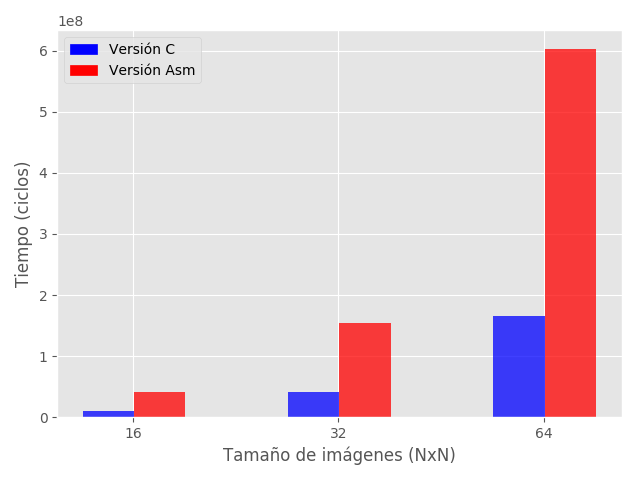
\includegraphics[width=0.8\textwidth]{imagenes/CvsAsm16-64.png}
\end{center}

\begin{center}
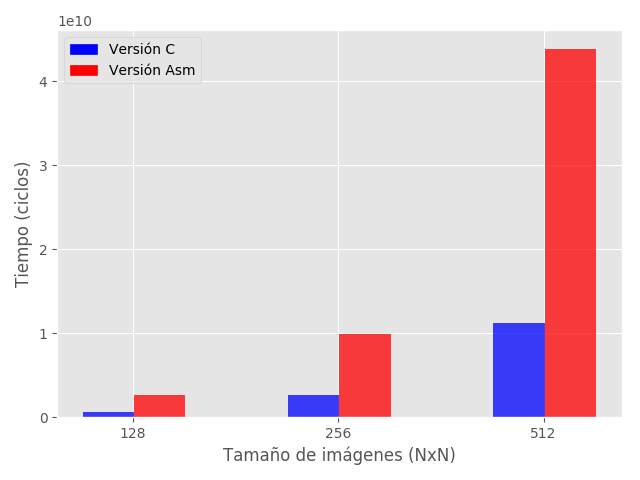
\includegraphics[width=0.8\textwidth]{imagenes/CvsAsm128-512.png}
\end{center}

En estos graficos se puede ver claramente que la implementacion en asm es mucho mas rapida y esta diferencia
crece aun más cuanto mas grande es la entrada. sin embargo en la proxima seccion se puede ver
en detalle como impacta en particular cada una de las funciones en el tiempo total.



\subsubsection{Una función en assembler a la vez}
Aqui se observa el tiempo de todo el programa de distintas formas, todo el codigo en C,
todo el codigo con solo una de las 3 funciones implementadas en asm y con dos casos para lin_solve
utilizando la version final (lin_solve) y la primera implementacion mas larga y compleja (lin_solve_largo)

\begin{center}
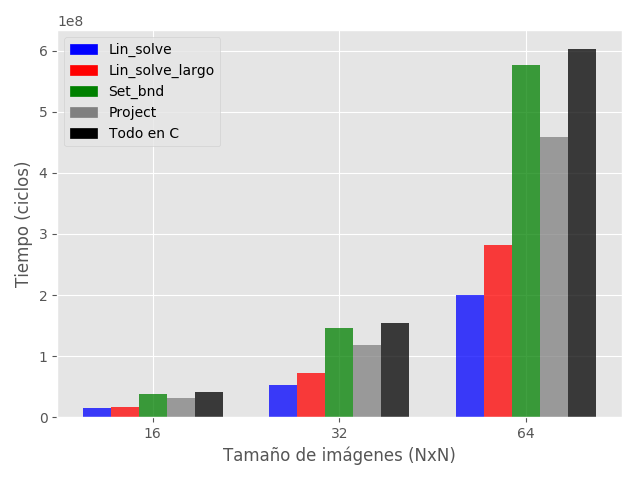
\includegraphics[width=0.8\textwidth]{imagenes/funciones16-64.png}
\end{center}

\begin{center}
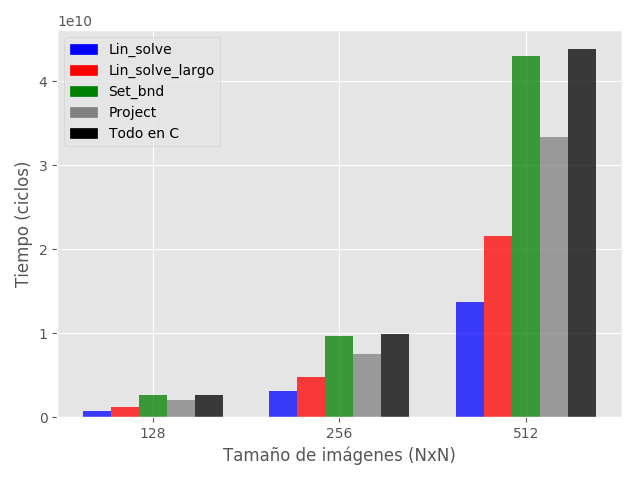
\includegraphics[width=0.8\textwidth]{imagenes/funciones128-512.png}
\end{center}

Analizando estos graficos, se puede ver que set_bnd, aunque presenta una mejoria, esta es infima
en comparacion a las otras funciones. Luego en el ranking viene project, la cual mejora el total del tiempo
pero aun asi ambas implementaciones de lin_solve representan la mayor parte de la mejoria de tiempo general.

Sindo lin_solve a su vez mejor que lin_solve_largo a pesar de que primero se creia lo contrario ya que
lin_solve_largo paraleliza mucho más y ejecuta menos ciclos. Sin embargo estos resultan más largos y aun más lentos en proporcion.

De aqui en adelante se trabaja con los tiempo medidos solo al principio y al final de la ejecucion de cada
funcion en particular en ambas implementaciones (C y asm) comparadas

\subsubsection{solver\_lin\_solve}
Se compara lin_solve final en asm contra lin_solve original en C.

\begin{center}
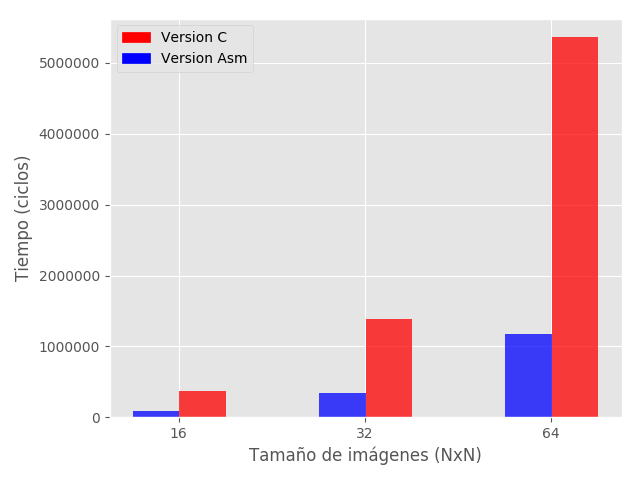
\includegraphics[width=0.8\textwidth]{imagenes/solver-lin-solve16-64.png}
\end{center}

\begin{center}
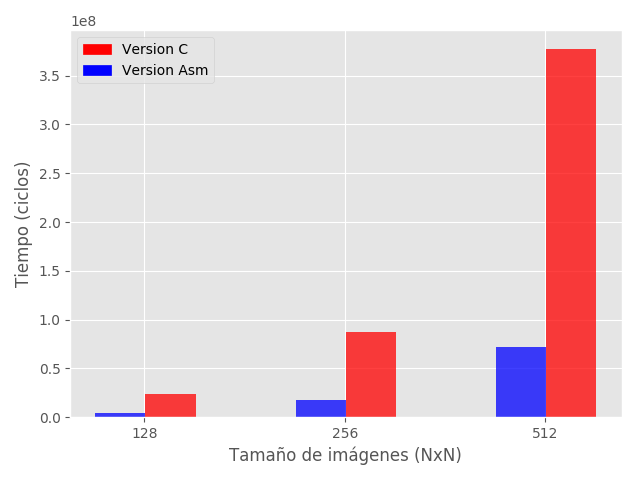
\includegraphics[width=0.8\textwidth]{imagenes/solver-lin-solve128-512.png}
\end{center}

Aqui se puede ver cuan abismal es la diferencia entre las versiones de lin_solve, cabe notar que nuestra
implementacion de lin_solve tiene un cambio en el orden de operaciones el cual facilita y acelera la ejecucion,
ademas de que el ciclo esta dividido en casos lo que reduce las comparaciones necesarias dentro del ciclo
y los simplifica sustancialmente.
Pero a pesar de ser matematicamente identica a la funcion original, el orden de operaciones afecta al
resultado final. Este tema sera visto con mejor detalle en la seccion diferencias.



\subsubsection{solver_set\_bnd}
Se compara set_bnd final en asm contra set_bnd original en C.

\begin{center}
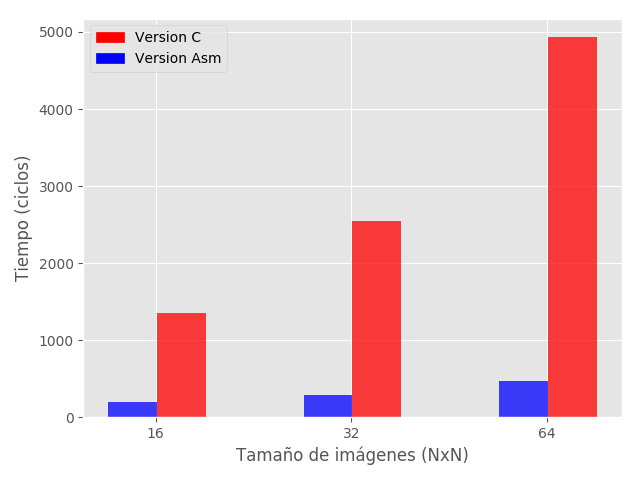
\includegraphics[width=0.8\textwidth]{imagenes/solver-set-bnd16-64.png}
\end{center}

\begin{center}
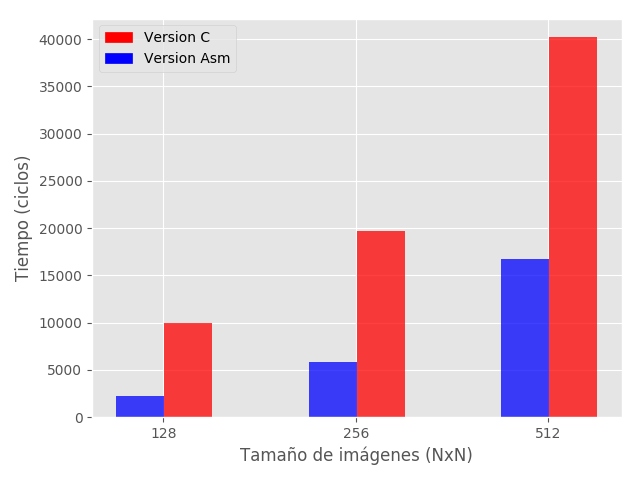
\includegraphics[width=0.8\textwidth]{imagenes/solver-set-bnd128-512.png}
\end{center}

Aqui se puede ver que set_bnd tambien presenta una buena mejora en asm respecto a C, pero notese que la escala
de tiempo es mucho más chica, lo cual muestra que la diferencia no significa mucho en cuanto al tiempo
total de la funcion, en otras palabras, la funcion set_bnd original ya ejecutaba pocos ciclos
en comparacion a las otras funciones y por eso la mejoria no es tan notable en lineas generales

\subsubsection{solver_project}
Se compara project final en asm contra project original en C.

\begin{center}
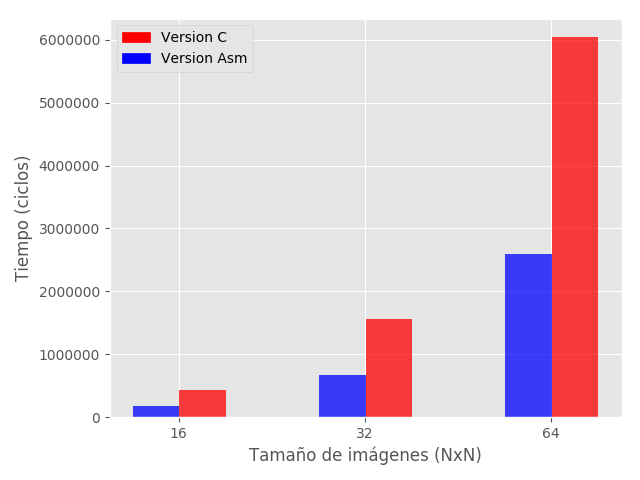
\includegraphics[width=0.8\textwidth]{imagenes/solver-project16-64.png}
\end{center}

\begin{center}
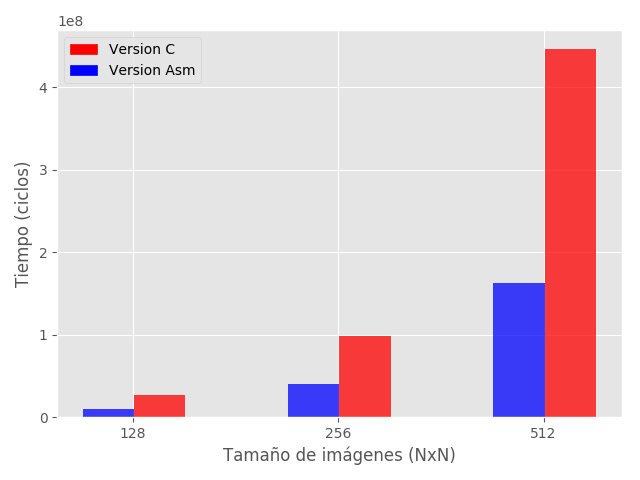
\includegraphics[width=0.8\textwidth]{imagenes/solver-project128-512.png}
\end{center}

Con project se puede ver que la implementacion en asm es muy buena en comparacion, pero la mejoria
es un poco menor que la que presenta lin_solve, y cuanto mas grande la entrada y al crecer exponencialmente
la diferencia entre C y asm,
mas se nota que lin_solve recude los tiempos en mayor medida, lo cual lleva a concluir
que lo visto en el primer grafico es acertado.





\subsection{Diferencias}

En esta seccion se observan las diferencias de las imagenes que corren los tests
en base a promedios y medianas.


Aqui se trabaja con todo el codigo en asm comparado al codigo original, notese que las
diferencias son en su totalidad causadas por la implementacion de lin_solve.


En primer lugar se decidio reescribir la funcion en C, modificando el orden de operacion
al realizar un factor comun, lo cual mantiene la logica matematica y facilita
la paralelizacion en asm y causa una mejoria temporal (como ya se vio en la seccion tiempo), pero introduce una diferencia
causada por el uso de floats, cuyos resultados si se ven afectados por el orden de operacion
sin importar la correctitud de la logica.
Entonces, ambos codigos en C (original y reescrito) ya presentaban una diferencia entre si.
Pero nuestra implementacion en asm, la cual se basa en la de C reescrita, no presenta ninguna diferencia
la misma, por lo cual decidimos mantener la implementacion como algo correcto.


No hay tablas para los tamaños de 16, 32 y 64 porque no hubo diferencias con las
versiones de la cátedra.

Promedio$_1$ es igual al promedio de todos los pixeles de la imagen

Promedio$_2$ es igual al promedio de solamente los píxeles que no son negros

Mediana$_1$ es igual a la mediana de todos los pixeles de la imagen

Mediana$_2$ es igual a la mediana de solamente los pixeles que no son negros

\begin{table}[H]
	\caption{Diferencias con la cátedra -- Tamaño $128\times128$} \label{tab:title}
	\begin{center}
		\begin{tabular}{| >{\centering\arraybackslash}m{0.9in} | >{\centering\arraybackslash}m{0.9in} | >{\centering\arraybackslash}m{0.9in} | >{\centering\arraybackslash}m{0.9in} |}
			\hline
			& \multicolumn{3}{c|}{\bf 128}\\
			\cline{2-4}
      & \bf Velocidad v & \bf Velocidad u & \bf Densidad \\\hline
      \bf Promedio$_1$ & 0.1113 & 0.9035 & 0.0015\\ \cline{2-4}
			\bf Promedio$_2$ & 1.0691 & 1.0096 & 1.0\\ \cline{2-4}
			\bf Mediana$_1$ & 0 & 1 & 0\\ \cline{2-4}
			\bf Mediana$_2$ & 1 & 1 & 1\\ \cline{2-4}
			\bf Cantidad & 1706 & 14662 & 25\\ \cline{2-4}
			\bf Maximo & 13 & 12 & 1\\ \cline{2-4}
			\hline
		\end{tabular}
	\end{center}
\end{table}

\begin{table}[H]
	\caption{Diferencias con la cátedra -- Tamaño $256\times256$} \label{tab:title}
	\begin{center}
		\begin{tabular}{| >{\centering\arraybackslash}m{0.9in} | >{\centering\arraybackslash}m{0.9in} | >{\centering\arraybackslash}m{0.9in} | >{\centering\arraybackslash}m{0.9in} |}
			\hline
			& \multicolumn{3}{c|}{\bf 256}\\
			\cline{2-4}
      & \bf Velocidad v & \bf Velocidad u & \bf Densidad \\\hline
      \bf Promedio$_1$ & 14.8418 & 0.0733 & 0.0740\\ \cline{2-4}
			\bf Promedio$_2$ & 14.8516 & 2.6657 & 9.9876\\ \cline{2-4}
			\bf Mediana$_1$ & 16 & 0 & 0\\ \cline{2-4}
			\bf Mediana$_2$ & 16 & 1 & 4\\ \cline{2-4}
			\bf Cantidad & 65493 & 1804 & 486\\ \cline{2-4}
			\bf Maximo & 105 & 39 & 129\\ \cline{2-4}
			\hline
		\end{tabular}
	\end{center}
\end{table}

\begin{table}[H]
	\caption{Diferencias con la cátedra -- Tamaño $512\times512$} \label{tab:title}
	\begin{center}
		\begin{tabular}{| >{\centering\arraybackslash}m{0.9in} | >{\centering\arraybackslash}m{0.9in} | >{\centering\arraybackslash}m{0.9in} | >{\centering\arraybackslash}m{0.9in} |}
			\hline
			& \multicolumn{3}{c|}{\bf 512}\\
			\cline{2-4}
      & \bf Velocidad v & \bf Velocidad u & \bf Densidad \\\hline
      \bf Promedio$_1$ & 1.5447 & 1.8360 & 0.1312\\ \cline{2-4}
			\bf Promedio$_2$ & 1.5721 & 1.8495 & 3.6362\\ \cline{2-4}
			\bf Mediana$_1$ & 1 & 2 & 0\\ \cline{2-4}
			\bf Mediana$_2$ & 1 & 2 & 2\\ \cline{2-4}
			\bf Cantidad & 257571 & 260225 & 9463\\ \cline{2-4}
			\bf Maximo & 61 & 30 & 48\\ \cline{2-4}
			\hline
		\end{tabular}
	\end{center}
\end{table}

De estas tablas se puede ver que, logicamente, cuanto mas grande la imagen mas pixeles distintos,
pero tambien se puede ver que estos pixeles distintos no alcanzan valores muy grandes, y las medianas
y los promedios se mantienen siempre muy bajo, lo cual marca que a pesar de haber diferencias, estas no son
abismales.


Pero extrañamente la matrix de 256 x 256 se comporta mucho peor que la de 512 x 512 más grande, esta ultima
presenta más pixeles con diferencias, pero la primera tiene diferencias mucho más grandes de hasta un poco sobre la mitad
del rango de color. Realmente no pudimos explicar este comportamiento.


Tambien se ve que la matriz densidad es por mucho la menos afectada en cantidad de pixeles distintos y en
diferencias en general, asumimos que esto se da porque la matriz de densidad pasa una sola vez por lin_solve por ciclo,
cuando las matrices de velocidad pasan almenos dos veces por lin_solve en cada ciclo.

\newpage
\section{Conclusión}

En concuclusion podemos decir que este trabajo nos permitio aprender y volcarnos en muchos aspectos distintos,
por ejemplo la programacion con SIMD y el procesamiento de matrices en assembler asi como en el desarrollo
de un informe profundo de experimentacion y analisis.


Se puede ver claramente lo que se buscaba sobre performance del programa
, ademas de poder justificarlo con pruebas y experimentos,
efectivamente se nota la mejora que causa el uso de la metodologia SIMD y assembler cuando se trata de
implementaciones que necesitan el procesamiento sistematico de muchos datos con caracteristicas iguales.


Tambien descubrimos con la implementacion de lin_solve (lin_solve_largo)
que no siempre más paralelizacion y mas trabajo por ciclo lleva a una mejoria temporal
sino que es mas importente aprovechar bien la logica de la memoria cache y no realizar
saltos lejanos en memoria en cada iteracion, como se penso en esta funcion en un principio.
Otro problema que encontramos fue que no se puedo sacar una conclusion clara de las tablas de diferencias
ni sobre por que los tests presentan el comportamiento particular mostrado en los resultados.
Quizas lo necesario seria mas conocimiento profundo sobre como trabaja el programa en general.


Cabe aclarar que este trabajo tambien sirvio como primer informe en la carrera de 2 integrantes del grupo, lo cual
aporto para lograr que sea una experiencia en la que se aprendio mucho sobre como se arman, revisan
y se desarrollan informes de investigacion.


\end{document}
